\documentclass[9pt]{article}
\usepackage[utf8]{inputenc}
\usepackage[german]{babel}
\usepackage{graphicx}
\usepackage{enumitem}
\usepackage{titlesec}
\usepackage{csquotes}
\usepackage{amsmath}
\usepackage{extsizes}
\usepackage[a4paper, margin=3.5cm]{geometry}

\makeatletter
\renewenvironment{abstract}{%
  \if@twocolumn
    \section*{\abstractname}
  \else
    \small
    \vspace*{-9mm}
    \begin{center}
    \end{center} 
    \quotation
  \fi
}
{
  \if@twocolumn
  \else
    \endquotation
  \fi
}
\makeatother

\titleformat{\section}
  {\normalfont\fontsize{11}{15}\bfseries}{\thesection.}{1em}{}

\title{\huge{\textbf{Bitcoin: Ein elektronisches Peer-to-Peer Geldsystem}}}
\author{\normalsize Satoshi Nakamoto\\ \normalsize satoshin@gmx.com\\ \normalsize www.bitcoin.org}
\date{}

\begin{document}

	\maketitle
	
	\begin{abstract}
		\noindent \textbf{Zusammenfassung.} \ Eine reine Peer-to-Peer-Version eines elektronischen Geldsystems würde es ermöglichen, Online-Zahlungen von einer Partei direkt an eine andere zu senden, ohne über ein Finanzinstitut zu gehen. Digitale Signaturen bilden einen Teil der Lösung, aber die Hauptvorteile gehen verloren, wenn weiterhin eine vertrauenswürdige dritte Partei notwendig ist, um Mehrfachausgaben zu verhindern. Wir schlagen eine Lösung für das Double-Spending-Problem (Problem der Mehrfachausgaben) vor, indem wir ein Peer-to-Peer-Netzwerk benutzen. Das Netzwerk gibt Transaktionen einen Zeitstempel, indem es diese in eine fortlaufende Kette von Hash-basierten Arbeitsbeweisen (Proof-of-Work) hasht. So erzeugt es eine Aufzeichnung, die nicht geändert werden kann, ohne den Proof-of-Work neu zu erzeugen. Die längste Kette dient nicht nur als Nachweis für die Sequenz bezeugter Ereignisse, sondern auch als Beweis, dass sie aus dem größten Pool an CPU-Leistung stammt. Solange der Großteil der CPU-Leistung von Nodes kontrolliert wird, die nicht kooperieren, um das Netzwerk anzugreifen, werden diese die längste Kette generieren und schneller sein als die Angreifer. Das Netzwerk selbst erfordert nur eine Minimalstruktur. Nachrichten werden nach bestem Wissen und Gewissen übertragen und die Nodes können das Netzwerk beliebig verlassen und wieder betreten, da sie die längste Proof-of-Work-Kette als Beweis darüber akzeptieren, was geschah, während sie weg waren.
	\end{abstract}
	
	\section{Einleitung}
	
	Der Internethandel stützt sich inzwischen fast vollständig auf Finanzinstitute, die bei der Abwicklung elektronischer Zahlungen als vertrauenswürdige Dritte dienen. Während dieses System für die meisten Transaktionen gut genug funktioniert, leidet es nach wie vor unter den Schwächen eines Modells, das auf Vertrauen beruht. Vollständig unumkehrbare Transaktionen sind nicht wirklich möglich, da Finanzinstitute nicht umhinkommen, in Streitfällen zu vermitteln. Die Kosten der Schlichtung erhöhen die Transaktionskosten, was die Mindestgröße für machbare Transaktionen einschränkt und die Möglichkeit kleiner Gelegenheitstransaktionen eliminiert. Ein größerer Schaden entsteht darüber hinaus durch den Wegfall der Möglichkeit, irreversible Zahlungen für irreversible Dienstleistungen zu tätigen. Durch die Option, Transaktionen rückgängig zu machen, wächst das Bedürfnis nach Vertrauen. Händler müssen ihren Kunden gegenüber misstrauisch sein und mehr Informationen von ihnen verlangen als sonst nötig wären. Ein bestimmtes Maß an Betrug wird als unvermeidbar akzeptiert. Diese Kosten- und Zahlungsunsicherheiten können durch persönlichen Kontakt und die Verwendung einer physischen Währung vermieden werden, doch es gibt keinen Mechanismus, um Zahlungen über einen Kommunikationskanal ohne vertrauenswürdige Partei durchzuführen. 

	Benötigt wird ein elektronisches Zahlungssystem, das auf kryptografischen Nachweisen an Stelle von Vertrauen basiert und zwei bereitwilligen Parteien ermöglicht, Transaktionen direkt und ohne eine dritte Partei untereinander durchzuführen. Transaktionen, die rechnerisch nicht rückgängig zu machen sind, würden Verkäufer vor Betrug schützen und zum Schutz der Käufer könnten standardisierte Treuhandmechanismen auf einfache Weise implementiert werden. In diesem Papier schlagen wir eine Lösung für das Double-Spending-Problem vor, die unter Verwendung eines verteilten Peer-to-Peer-Zeitstempel-Servers einen rechnerischen Nachweis über die chronologische Reihenfolge der Transaktionen erzeugt. Das System ist sicher, solange die ehrlichen Nodes mehr CPU-Leistung kontrollieren als jede kooperierende Gruppe von angreifenden Nodes.
	
	\newpage
	
	\section{Transaktionen}
	Wir definieren eine elektronische Münze (Coin) als eine Kette digitaler Signaturen. Jeder Eigentümer überträgt den Coin auf den nächsten, indem er einen Hash der vorherigen Transaktion sowie den öffentlichen Schlüssel des nächsten Eigentümers digital signiert und dies an das Ende des Coins anhängt. Der Empfänger der Zahlung kann die Signaturen verifizieren, um die Kette der Eigentümer nachzuvollziehen.
	
	\begin{center}
		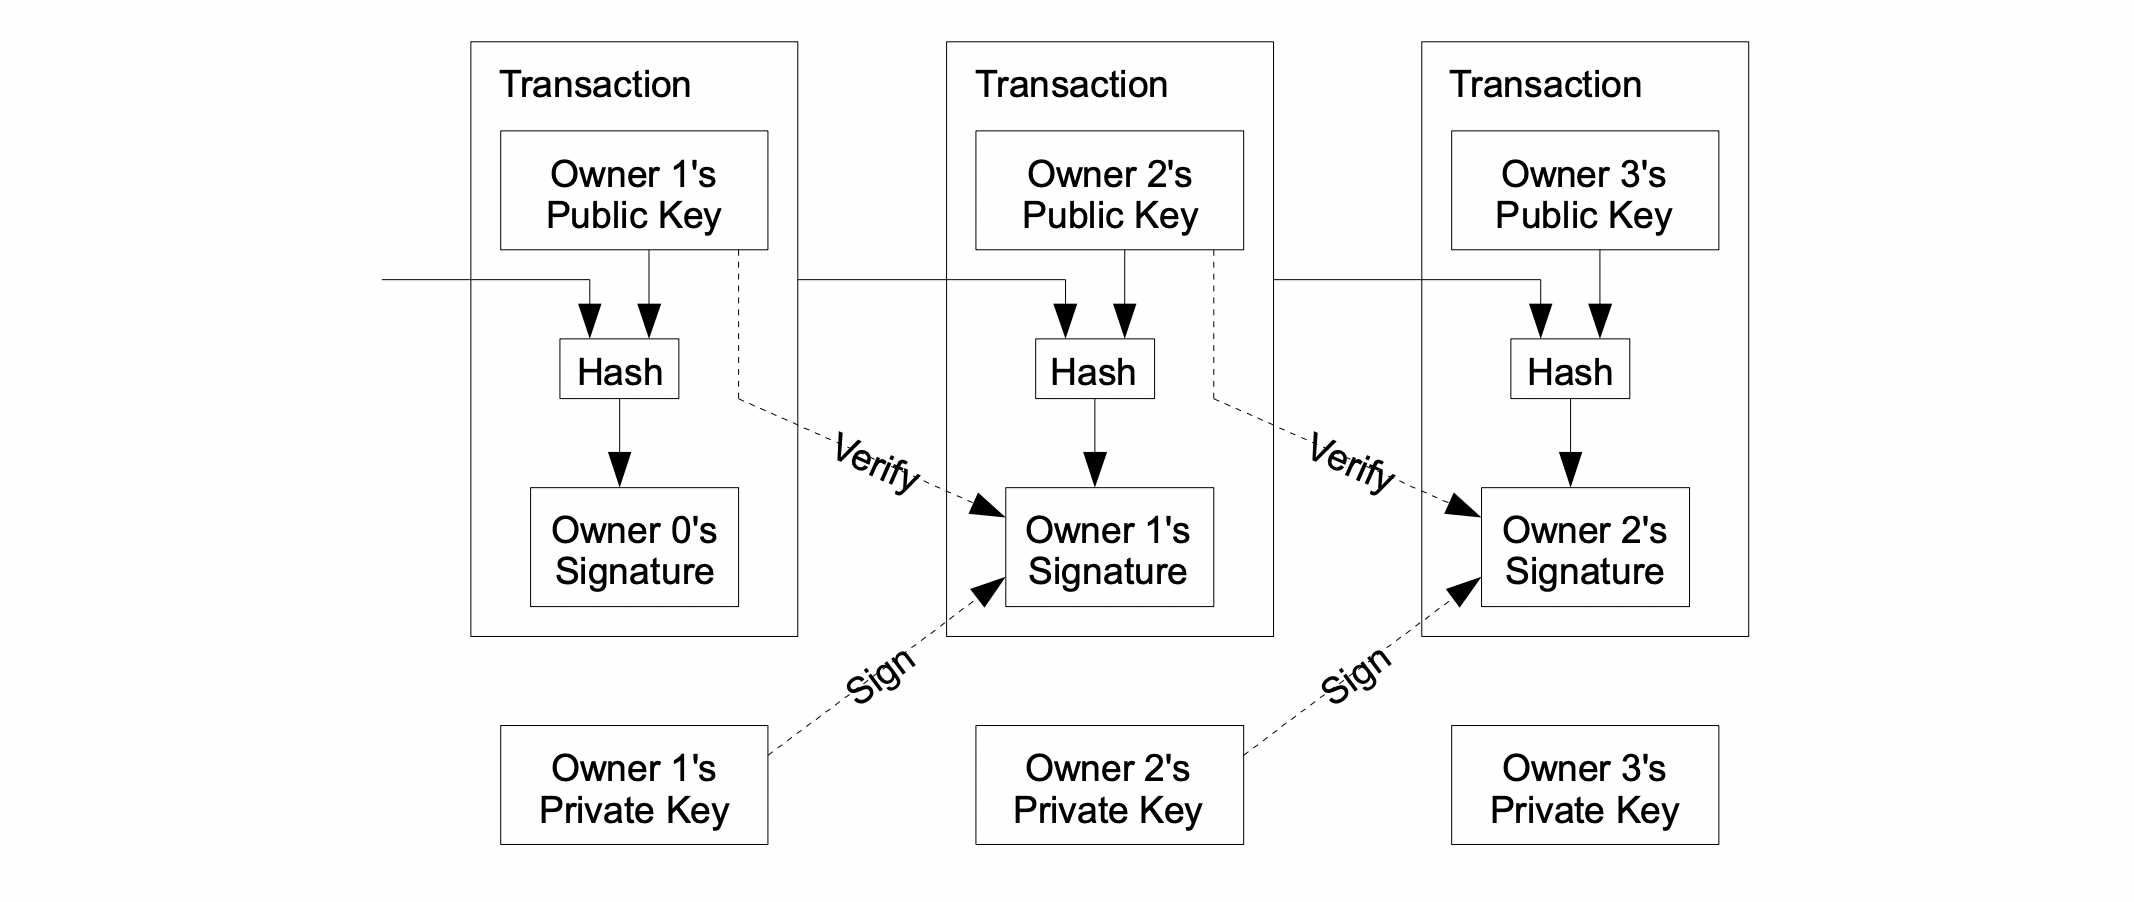
\includegraphics[width=\textwidth]{pics/transactions.png}		
	\end{center}

	Das Problem ist natürlich, dass der Zahlungsempfänger nicht verifizieren kann, dass einer der Eigentümer den Coin nicht doppelt ausgegeben hat. Eine gängige Lösung ist, eine zentrale, vertrauenswürdige Instanz, oder Münzanstalt, einzuführen, die jede Transaktion auf Double-Spending (Mehrfachausgabe) prüft. Nach jeder Transaktion muss der Coin an die Instanz zurückgegeben werden, damit diese einen neuen Coin herausgibt. Nur bei Coins, die direkt von der Instanz ausgegeben wurden, kann darauf vertraut werden, dass sie nicht doppelt ausgegeben wurden. Das Problem an dieser Lösung ist, dass das Schicksal des gesamten Geldsystems von dem Unternehmen abhängt, das die Münzanstalt betreibt und dass jede Transaktion über dieses laufen muss, wie bei einer Bank.
	
	Wir benötigen daher eine Methode, um Gewissheit für den Zahlungsempfänger darüber zu schaffen, dass die vorherigen Eigentümer keine früheren Transaktionen signiert haben. Für unsere Zwecke ist die erste Transaktion diejenige, die zählt, sodass wir uns keine Sorgen über spätere Versuche zur Mehrfachausgabe machen müssen. Die einzige Möglichkeit, die Abwesenheit einer Transaktion zu bestätigen, ist es, alle Transaktionen zu kennen. In dem auf einer Münzanstalt basierenden Modell kannte die Münzanstalt alle Transaktionen und konnte entscheiden, welche zuerst eingetroffen ist. Um dies ohne vertrauenswürdige Partei zu erreichen, müssen Transaktionen öffentlich gemacht werden \cite{dai} und wir benötigen ein System, mit dem sich die Teilnehmer auf einen einheitlichen Verlauf der Reihenfolge einigen, in der sie eingetroffen sind. Der Zahlungsempfänger benötigt einen Nachweis darüber, dass zum Zeitpunkt jeder Transaktion die Mehrheit der Nodes innerhalb des Netzwerks zugestimmt hat, dass diese zuerst empfangen wurde.

	\section{Zeitstempel-Server}
	
    Die von uns vorgeschlagene Lösung beginnt mit einem Zeitstempel-Server. Ein Zeitstempel-Server funktioniert, indem er den Hash eines mit einem Zeitstempel zu versehenden Blockes nimmt und den Hash weitläufig, etwa in einer Zeitung oder in einem Usenet-Post, veröffentlicht [2-5]. Der Zeitstempel beweist, dass die Daten zu diesem Zeitpunkt bereits existiert haben müssen, denn sonst gäbe es keinen Hash von ihnen. Jeder Zeitstempel beinhaltet in seinem Hash den vorhergegangenen Zeitstempel und bildet eine Kette, bei der jeder zusätzliche Zeitstempel die vorherigen bekräftigt.
    
	\begin{center}
		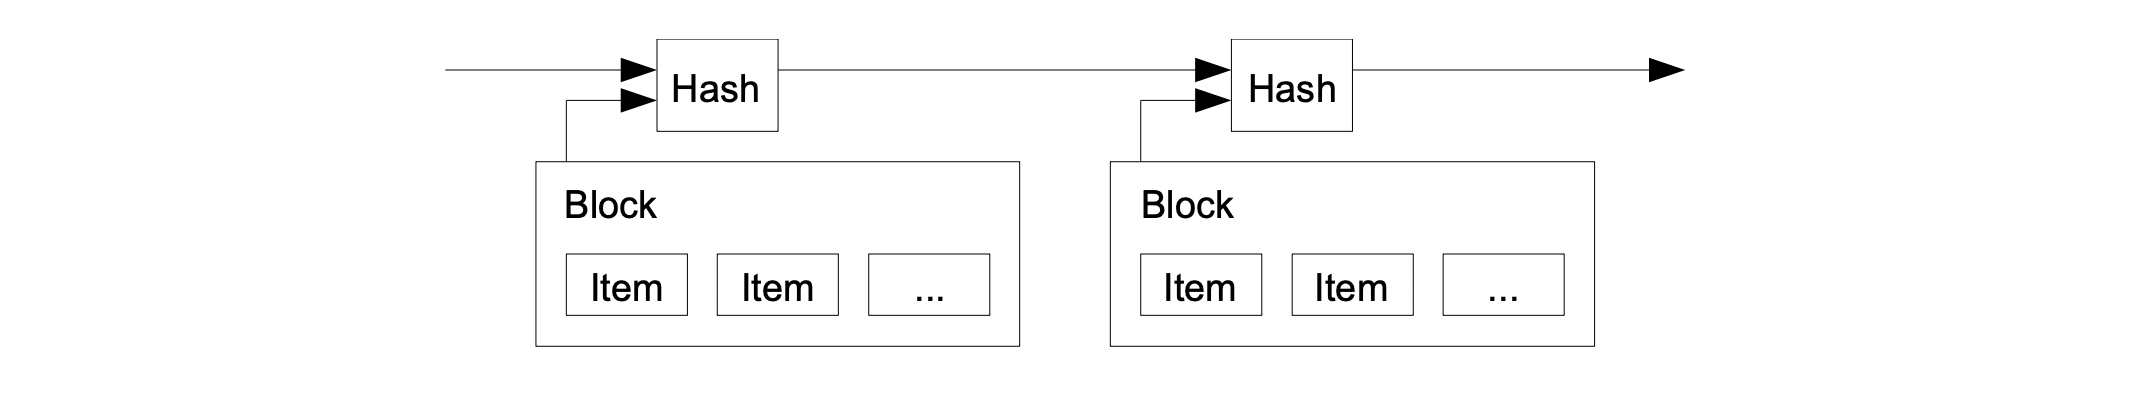
\includegraphics[width=.9\textwidth]{pics/timestampserver.png}
	\end{center}

	\newpage
	
	\section{Proof-of-Work}
	
	Um einen verteilten Zeitstempel-Server auf Peer-to-Peer-Basis zu implementieren, müssen wir ein Proof-of-Work-System, ähnlich des Hashcash-Systems von Adam Back [6] verwenden statt Zeitungen oder Usenet-Posts. Beim Proof-of-Work wird nach einem Wert gesucht, bei dem, wenn er gehasht wird, etwa durch SHA-256, der Hash mit einer Anzahl von Nullbits beginnt. Der durchschnittliche Arbeitsaufwand ist exponentiell zur Anzahl der erforderlichen Nullbits und kann durch die Ausführung eines einzelnen Hashs verifiziert werden.
	
    Für unser Zeitstempel-Netzwerk implementieren wir den Proof-of-Work, indem eine Nonce im Block so lange ansteigt, bis ein Wert gefunden wird, der dem Hash des Blocks die erforderlichen Nullbits gibt. Nachdem die CPU genügend Arbeit aufgewendet hat, um den Proof-of-Work zu erfüllen, kann der Block nicht mehr geändert werden, ohne dass die Arbeit erneut ausgeführt wird. Da spätere Blöcke damit verkettet werden, würde die Arbeit zur Änderung des Blocks die Neuerstellung aller nachfolgenden Blocks beinhalten.
	
	\begin{center}
		
\includegraphics[width=\textwidth]{pics/proofofwork.png}	
	\end{center}
	
	Der Proof-of-Work löst außerdem das Problem, bei Mehrheitsentscheidungen die Repräsentanten zu bestimmen. Würde die Mehrheit auf einer Stimme je IP-Adresse basieren, könnte diese durch jeden unterwandert werden, der in der Lage ist, mehrere IPs zu reservieren. Proof-of-Work ist im Grunde eine Stimme pro CPU. Die Mehrheitsentscheidung wird durch die längste Kette repräsentiert, in die der größte Proof-of-Work-Aufwand investiert wurde. Wenn eine Mehrheit der CPU-Leistung von ehrlichen Nodes kontrolliert wird, wächst die ehrliche Kette am schnellsten und hängt alle konkurrierenden Ketten ab. Um einen vergangenen Block zu ändern, müsste ein Angreifer den Proof-of-Work des Blocks sowie den aller nachfolgenden Blocks neu erzeugen und dann die ehrlichen Nodes überholen. Wir werden später demonstrieren, dass die Wahrscheinlichkeit, dass ein langsamerer Angreifer aufholt, exponentiell abnimmt, je mehr nachfolgende Blöcke hinzugefügt werden.

    Um steigende Hardwareleistung und zeitlich schwankendes Interesse daran, eine arbeitende Node zu betreiben, auszugleichen, wird die Proof-of-Work-Schwierigkeit durch einen gleitenden Mittelwert bestimmt, der auf eine durchschnittliche Anzahl von Blöcken pro Stunde abzielt. Wenn sie zu schnell generiert werden, steigt die Schwierigkeit.
	
	\section{Netzwerk}
	
    Dies sind die Schritte zum Betrieb des Netzwerks:
	
	\begin{enumerate}[label={\arabic*)}, topsep=0pt, itemsep=-1ex, partopsep=1ex, parsep=1ex]
		\item Neue Transaktionen werden an alle Nodes übertragen.
		\item Jede Node sammelt die neuen Transaktionen in einem Block.
		\item Jede Node arbeitet daran, einen schwierigen Proof-of-Work für ihren Block zu finden.
		\item Wenn eine Node einen Proof-of-Work findet, überträgt sie den Block an alle Nodes.
		\item Die Nodes akzeptieren den Block nur, wenn alle Transaktionen darin gültig sind und nicht bereits ausgegeben wurden.
		\item Die Nodes drücken ihre Akzeptanz des Blocks aus, indem sie an der Erstellung des nächsten Blocks in der Kette arbeiten. Dabei wird der Hash des akzeptierten Blocks als vorheriger Hash verwendet.
	\end{enumerate}
	
	Nodes gehen immer davon aus, dass die längste Kette die korrekte ist und arbeiten daran, diese zu verlängern. Wenn zwei Nodes gleichzeitig verschiedene Versionen des nächsten Blocks übertragen, können einige Nodes die eine oder die andere Version zuerst empfangen. In diesem Fall arbeiten sie an der ersten, die sie empfangen haben, speichern aber den anderen Zweig für den Fall, dass dieser länger wird. Der Gleichstand wird gebrochen, wenn der nächste Proof-of-Work gefunden wird und ein Zweig länger wird; die Nodes, die am anderen Zweig gearbeitet haben, werden dann auf den längeren umschalten.

	\newpage
	
	Die Übertragung neuer Transaktionen muss nicht zwingend jede Node erreichen. Solange sie viele Nodes erreichen, werden sie früher oder später in einem Block aufgenommen. Blockübertragungen sind auch tolerant gegenüber verlorenen Nachrichten. Wenn eine Node einen Block nicht empfängt, wird sie diesen anfordern, sobald sie den nächsten Block empfängt und erkennt, dass ihr einer fehlt.
		
	\section{Anreize}
	
	Konventionell ist die erste Transaktion in einem Block eine spezielle Transaktion. Sie schöpft einen neuen Coin, der dem Erzeuger des Blocks gehört. Dies gibt neuen Nodes einen Anreiz, das Netzwerk zu unterstützen und bietet einen Weg, Münzen erstmals in Umlauf zu bringen, da es keine zentrale Instanz gibt, die sie herausgibt. Das ständige Hinzufügen einer konstanten Anzahl neuer Coins ist analog zu Goldgräbern, die Ressourcen aufwenden, um mehr Gold in Umlauf zu bringen. In unserem Falle sind es CPU-Zeit und Elektrizität, die aufgewendet werden.

    Die Anreize können auch durch Transaktionsgebühren gefördert werden. Ist der Ausgangswert der Transaktion geringer als ihr Eingangswert, wird die Differenz als Transaktionsgebühr zur Belohnung des Blocks addiert, der die Transaktion enthält. Wurde einmal eine vorherbestimmte Anzahl an Coins in Umlauf gebracht, können die Anreize vollständig auf Transaktionsgebühren übergehen und so vollständig inflationsfrei sein.

    Die Anreize können helfen, Nodes zu motivieren, ehrlich zu bleiben. Wenn ein gieriger Angreifer in der Lage ist, mehr CPU-Leistung aufzubringen als alle ehrlichen Nodes, müsste er sich entscheiden: Verwendet er diese Leistung, um Menschen zu betrügen, indem er seine Zahlungen zurück stiehlt, oder verwendet er sie, um neue Coins zu erzeugen. Für ihn sollte es profitabler sein, sich an die Regeln zu halten — Regeln, die ihn mit mehr neuen Coins versorgen können als alle anderen zusammen — als das System und damit die Gültigkeit seines eigenen Wohlstands zu untergraben.

	\section{Speicherplatz zurück gewinnen}
	
	Sobald die letzte Transaktion eines Coins unter ausreichend Blöcken begraben ist, können die verbrauchten Transaktionen davor gelöscht werden, um Speicherplatz zu sparen. Um dies zu ermöglichen, ohne den Hash des Blocks zu brechen, werden die Transaktionen in einem Merkle-Tree \cite{merkle}\cite{massias}\cite{haber2} gehasht. Lediglich die Wurzel wird in den Hash des Blocks aufgenommen. Alte Blöcke können dann komprimiert werden, indem Zweige des Merkle-Trees gekappt werden. Die internen Hashes müssen nicht gespeichert werden.
	
	\begin{center}
		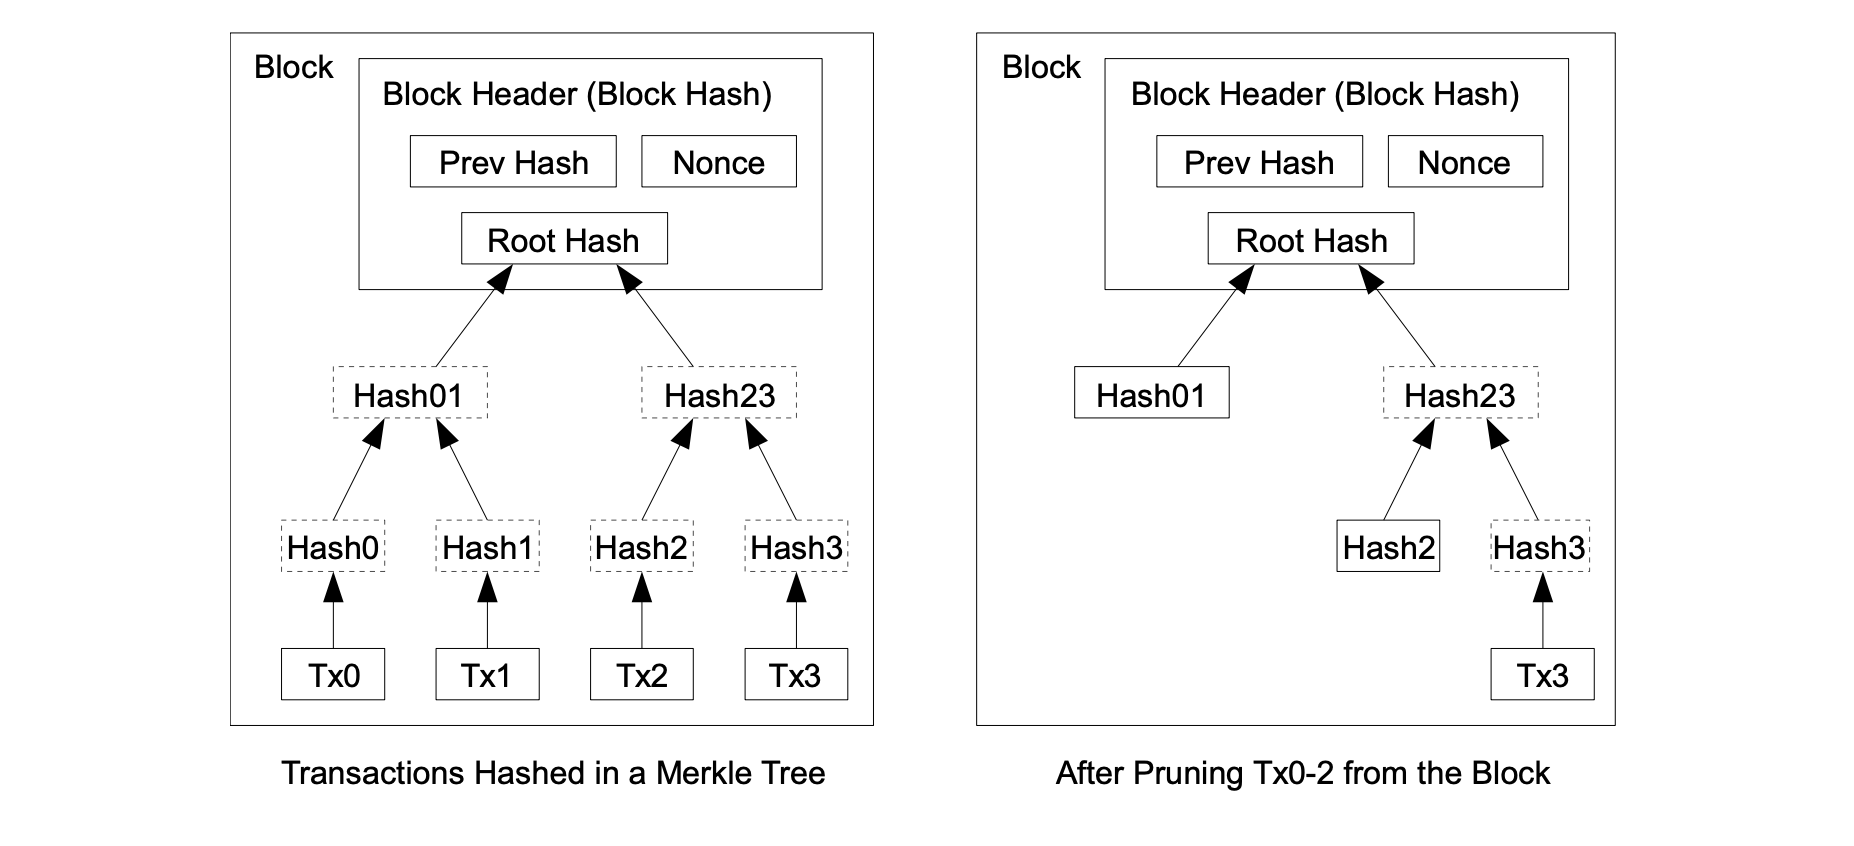
\includegraphics[width=\textwidth]{pics/reclaimingdiskspace.png}
	\end{center}
	
	Ein Blockheader ohne Transaktionen benötigt etwa 80 Byte. Wenn wir davon ausgehen, dass Blöcke alle 10 Minuten generiert werden, entsprechen 80 Byte $* \;6 * 24 * 365 = 4,2$ MB pro Jahr. Mit Computersystemen, die im Jahr (Stand 2008) typischerweise mit 2 GB RAM verkauft werden und Moores Law, das aktuell ein Wachstum von 1,2 GB prognostiziert, sollte Speicherplatz kein Problem darstellen, selbst wenn die Blockheader im Speicher gehalten werden müssen.
	
	\newpage
	
	\section{Vereinfachte Zahlungsverifizierung}
	
    Zahlungen können verifiziert werden, ohne eine kompletten Node im Netzwerk zu betreiben. Ein Nutzer muss lediglich eine Kopie der Blockheader der längsten Proof-of-Work-Kette aufbewahren. Diese erhält er, indem er andere Nodes so lange abfragt, bis er überzeugt ist, dass er die längste Kette hat und den Merkle-Tree-Zweig bezieht, der die Transaktion mit dem Block verknüpft, durch den sie einen Zeitstempel erhalten hat. Er kann die Transaktion nicht selbst prüfen. Aber indem er sie mit einer Stelle in der Kette verknüpft, kann er sehen, dass sie von einem Netzwerk-Knoten akzeptiert wurde. Blöcke, die danach angefügt wurden, bestätigen weiter, dass sie vom Netzwerk akzeptiert wurde.
	
	\begin{center}
		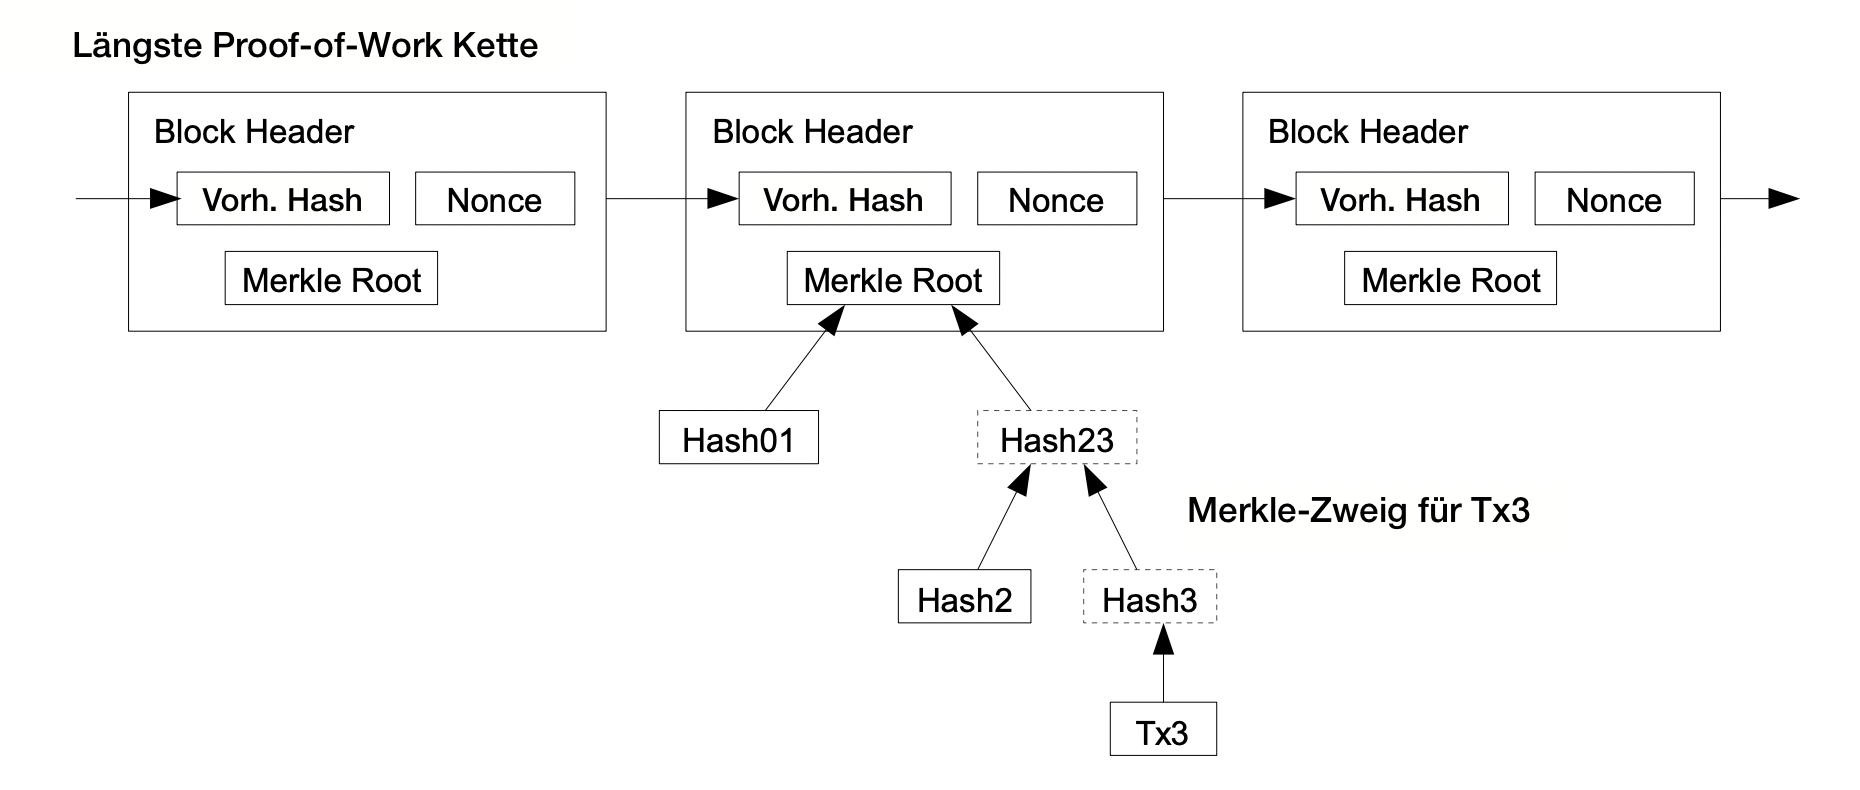
\includegraphics[width=\textwidth]{pics/spv.png}
	\end{center}
	
    Die Verifizierung ist also zuverlässig, solange ehrliche Nodes das Netzwerk kontrollieren. Sie wird jedoch angreifbarer, wenn das Netzwerk von einem Angreifer überwältigt wird. Während Netzwerk-Knoten Transaktionen selbst verifizieren können, kann die vereinfachte Methode so lange durch einen Angreifer mit fingierten Transaktionen getäuscht werden, wie der Angreifer das Netzwerk dominieren kann. Eine Strategie, sich dagegen zu schützen, liegt darin, Alarmsignale von Netzwerk-Nodes zu akzeptieren, wenn diese einen ungültigen Block erkennen. Das würde die Software des Users dazu veranlassen, den vollen Block und die vom Alarm betroffenen Transaktionen herunterzuladen, um die Inkonsistenz zu bestätigen. Unternehmen, die regelmäßige Zahlungen erhalten, werden dennoch ihre eigenen Nodes betreiben wollen, für eine unabhängigere Sicherheit und schnellere Verifizierung.

	\section{Zusammenführung und Aufteilung von Werten}
	
    Obgleich es möglich wäre, Coins einzeln zu behandeln, wäre es unpraktisch, für jeden Cent einer Überweisung eine separate Transaktion durchzuführen. Damit Werte aufgeteilt und zusammengeführt werden können, enthalten Transaktionen mehrere Ein- und Ausgänge. Normalerweise gibt es entweder einen einzelnen Input von einer größeren vorausgegangenen Transaktion oder mehrere Eingänge, die kleinere Beträge zusammenfassen. Daneben gibt es höchstens zwei Ausgänge: einen für die Zahlung und einen, der das Wechselgeld, falls vorhanden, an den Absender zurückgibt.
	
	\begin{center}
		
\includegraphics[width=\textwidth]{pics/combineandsplit.png}
	\end{center}
	
    Zu beachten ist, dass ein Fan-Out, bei dem eine Transaktion von mehreren Transaktionen abhängt und diese wiederum von vielen anderen Transaktionen abhängen, in diesem Fall kein Problem darstellt. Es besteht niemals die Notwendigkeit, eine vollständige Kopie eines Transaktionsverlaufs abzurufen.	
    
	\newpage
	
	\section{Privatsphäre}
	
    Das traditionelle Bankenmodell erreicht ein bestimmtes Datenschutzniveau, indem der Zugriff auf die Informationen auf die beteiligten Parteien und die vertrauenswürdige dritte Partei begrenzt wird. Die Notwendigkeit, alle Transaktionen öffentlich bekannt zu machen, schließt diese Methode aus. Der Datenschutz kann dennoch aufrechterhalten werden, indem der Informationsfluss an anderer Stelle unterbrochen wird: indem die öffentlichen Schlüssel anonym bleiben. Die Öffentlichkeit kann sehen, dass jemand einen Betrag an jemand anderen sendet, jedoch ohne Informationen, die die Transaktionen mit jemandem in Verbindung bringen. Das ist vergleichbar mit den Informationen, die von Aktienbörsen veröffentlicht werden: Zeit und Umfang der einzelnen Geschäfte und das \enquote{Tape} werden veröffentlicht, ohne die Parteien zu nennen.	

	\begin{center}
		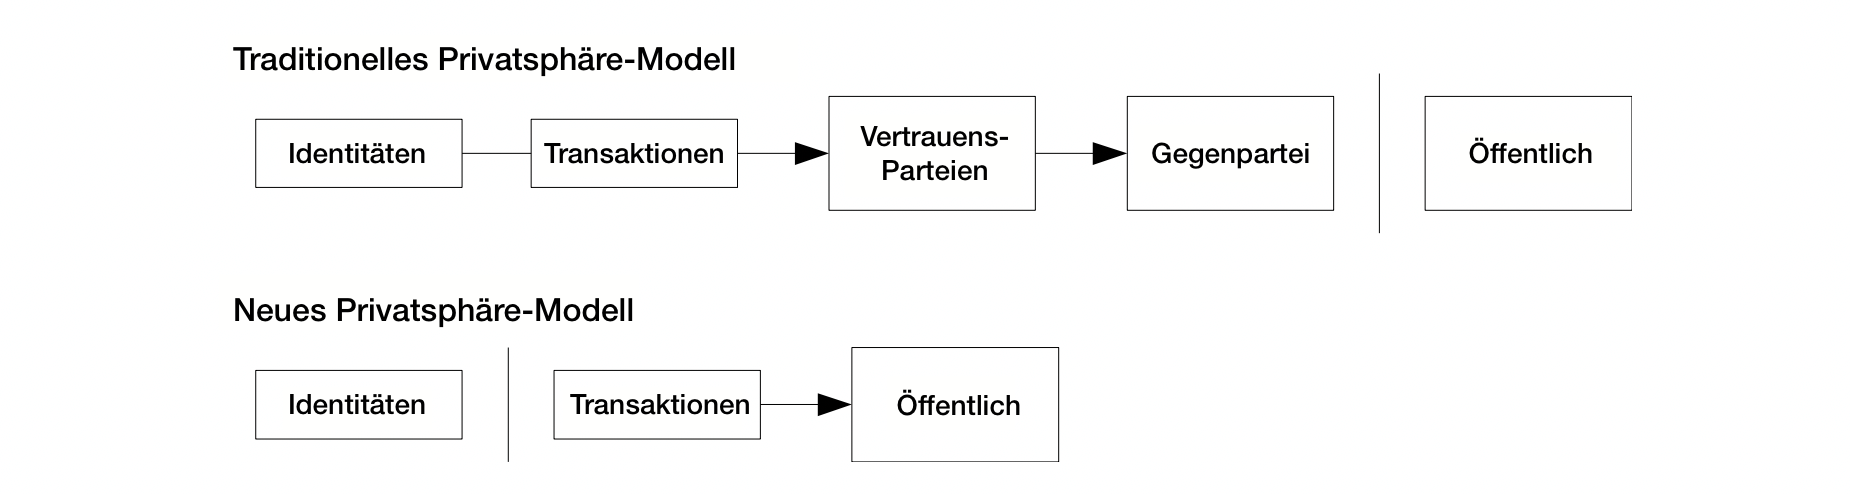
\includegraphics[width=\textwidth]{pics/privacy.png}
	\end{center}
	
    Als zusätzlicher Schutzwall sollte für jede Transaktion ein neues Schlüsselpaar verwendet werden, um zu vermeiden, dass die Schlüssel einem Eigentümer zugeordnet werden können. Manche Verknüpfungen sind bei Transaktionen mit mehreren Eingängen noch immer unvermeidbar, weil diese notwendigerweise preisgeben, dass ihre Eingänge zum gleichen Eigentümer gehören. Das Risiko besteht darin, dass bei Bekanntwerden des Eigentümers eines Schlüssels die Verbindung zu anderen Transaktionen desselben Eigentümers aufgedeckt werden könnte.
	
	\section{Berechnungen}
	
	Betrachten wir ein Szenario, bei dem ein Angreifer versucht, eine alternative Kette schneller zu erzeugen als die ehrliche Kette. Selbst wenn dies gelingt, ist das System nicht anfällig für willkürliche Änderungen, wie zum Beispiel die Erzeugung von Wert aus dem Nichts oder die Entnahme von Geld, das dem Angreifer nicht gehört. Die Nodes werden keine ungültige Transaktion als Zahlung akzeptieren und die ehrlichen Nodes werden niemals einen Block akzeptieren, der eine solche enthält. Ein Angreifer kann lediglich versuchen, eine seiner eigenen Transaktionen zu verändern, um Geld zurückzubekommen, das er vor kurzem ausgegeben hat.
	
	Der Wettlauf zwischen einer ehrlichen Kette und der Kette eines Angreifers kann als binomischer Random Walk charakterisiert werden. Das Erfolgsereignis ist die Erweiterung der ehrlichen Kette um einen Block, wodurch sich deren Vorsprung um $+1$ erhöht. Das Scheitern liegt in der Erweiterung der Kette des Angreifers um einen Block, wodurch sich der Abstand um $-1$ verringert.
        
    Die Wahrscheinlichkeit, dass ein Angreifer einen Rückstand aufholt, entspricht dem Problem des \enquote{Ruin des Spielers}. Angenommen, ein Spieler mit unbegrenztem Kredit beginnt mit einem Rückstand und spielt eine potenziell unendliche Anzahl von Partien, mit dem Ziel, die Gewinnschwelle zu erreichen. Wir können die Wahrscheinlichkeit, dass er jemals die Gewinnschwelle erreicht, oder dass ein Angreifer jemals eine ehrliche Kette einholt, wie folgt berechnen \cite{feller}:
	
	\vspace{2mm}
	\indent $p =$ Wahrscheinlichkeit, dass eine ehrliche Node den nächsten Block findet\\
	\indent $q =$ Wahrscheinlichkeit, dass der Angreifer den nächsten Block findet\\
	\indent $q_z =$ Wahrscheinlichkeit, dass der Angreifer jemals den Rückstand von $z$ Blöcken aufholt

	\begin{flalign*}
\indent q_z = 
	\begin{cases}
		1 & \text{if} \ p \leq q \\
		(q/p)^z & \text{if} \ p > q
	\end{cases}
\Biggl\} &&
	\end{flalign*}
	
	\newpage
	
	Unter unserer Annahme, dass $p > q$, fällt die Wahrscheinlichkeit exponentiell, wenn die Anzahl der Blöcke, die der Angreifer aufholen muss, steigt. Wenn er nicht frühzeitig einen erfolgreichen Sprung vorwärtsmacht, werden seine Chancen schwindend gering, je weiter er zurückfällt.

    Wir wollen nun untersuchen, wie lange der Empfänger einer neuen Transaktion warten muss, bevor er sich sicher sein kann, dass der Absender die Transaktion nicht mehr ändern kann.  Nehmen wir an, der Absender ist ein Angreifer, der den Empfänger für eine Weile glauben lassen möchte, er wurde bezahlt. Nach einiger Zeit verändert er dann die Transaktion, sodass sie an ihn selbst zurückgezahlt wird. Der Empfänger wird alarmiert, wenn dies geschieht, der Absender hofft jedoch, dass es dann zu spät ist.

    Der Empfänger generiert ein neues Schlüsselpaar und gibt den Public Key kurz vor dem Signieren an den Sender. Dies verhindert, dass der Sender bereits im Voraus eine Kette von Blocks vorbereitet, indem er so lange daran arbeitet, bis er das Glück hat, weit genug voraus zu sein, und die Transaktion dann in diesem Moment ausführt. Sobald die Transaktion abgeschickt wurde, beginnt der unehrliche Sender insgeheim mit der Arbeit an einer parallelen Kette, die eine geänderte Version seiner Transaktion enthält.

    Der Empfänger wartet, bis die Transaktion zu einem Block hinzugefügt wurde und $z$ Blöcke dahinter angefügt wurden. Den genauen Fortschritt des Angreifers kennt er nicht. Geht man aber davon aus, dass die ehrlichen Blöcke die durchschnittliche Zeit pro Block benötigt haben, entspricht der potenzielle Fortschritt des Angreifers einer Poisson-Verteilung mit dem erwarteten Wert:
	
	\begin{flalign*}
\indent \lambda = z \ \frac{q}{p} &&
	\end{flalign*}
	\vspace{2mm}
	
	\noindent Um die Wahrscheinlichkeit zu ermitteln, mit der der Angreifer jetzt noch aufholen könnte, multiplizieren wir die Poisson-Dichte für jede Summe des Fortschritts, den er gemacht haben könnte, mit der Wahrscheinlichkeit, dass er von diesem Punkt an aufholen könnte:
	
	\begin{flalign*}
\indent \sum_{k = 0}^{\infty} \frac{\lambda^k e^{-\lambda}}{k!} \cdot 
	\begin{cases}
		(q/p)^{(z-k)} & \text{if} \ k \leq z\\
		1 & \text{if} \ k > z
	\end{cases}
\Biggl\}&&
	\end{flalign*}
	\vspace{2mm}
	
	\noindent Wir stellen die Formel um, um zu vermeiden, dass die unendlichen Nachkommastellen der Verteilung addiert werden…
	
	\begin{flalign*}
\indent 1 - \sum_{k = 0}^{z} \frac{\lambda^k e^{-\lambda}}{k!} (1- (q/p)^{(z-k)})&&
	\end{flalign*}
	\vspace{2mm}
	
	\noindent Umwandlung in C-Code...
	
	\begin{verbatim}
#include <math.h>
double AttackerSuccessProbability(double q, int z)
{
    double p = 1.0 - q;
    double lambda = z * (q / p);
    double sum = 1.0;
    int i, k;
    for (k = 0; k <= z; k++)
    {
        double poisson = exp(-lambda);
        for (i = 1; i <= k; i++)
            poisson *= lambda / i;
        sum -= poisson * (1 - pow(q / p, z - k));
    }
    return sum;
}
	\end{verbatim}
	
	\newpage
	
	\noindent Wenn wir einige Ergebnisse durchlaufen lassen, können wir erkennen, dass die Wahrscheinlichkeit exponentiell mit $z$ abfällt.
	
	\begin{verbatim}
  q=0.1
  z=0    P=1.0000000
  z=1    P=0.2045873
  z=2    P=0.0509779
  z=3    P=0.0131722
  z=4    P=0.0034552
  z=5    P=0.0009137
  z=6    P=0.0002428
  z=7    P=0.0000647
  z=8    P=0.0000173
  z=9    P=0.0000046
  z=10   P=0.0000012

  q=0.3
  z=0    P=1.0000000
  z=5    P=0.1773523
  z=10   P=0.0416605
  z=15   P=0.0101008
  z=20   P=0.0024804
  z=25   P=0.0006132
  z=30   P=0.0001522
  z=35   P=0.0000379
  z=40   P=0.0000095
  z=45   P=0.0000024
  z=50   P=0.0000006
	\end{verbatim}
	
	\noindent Auflösung für $P$ kleiner als $0.1\%$ …
	
	\begin{verbatim}
  P < 0.001
  q=0.10 z=5
  q=0.15 z=8
  q=0.20 z=11
  q=0.25 z=15
  q=0.30 z=24
  q=0.35 z=41
  q=0.40 z=89
  q=0.45 z=340
	\end{verbatim}
	
	\section{Fazit}
	
    Wir haben ein System für elektronische Transaktionen vorgeschlagen, das sich nicht auf Vertrauen stützt. Wir sind vom üblichen System von aus digitalen Signaturen erstellten Coins ausgegangen. Dieses bietet eine starke Kontrolle der Eigentumsverhältnisse, ist aber unvollständig ohne eine Möglichkeit, doppelte Ausgaben zu verhindern. Um dieses Problem zu lösen, haben wir ein Peer-to-Peer-Netzwerk vorgeschlagen, das Proof-of-Work verwendet, um eine öffentliche  Transaktionshistorie aufzuzeichnen, die für Angreifer unmöglich veränderbar ist, solange ehrliche Nodes die Mehrheit der CPU-Leistung kontrollieren. Das Netzwerk ist in seiner unstrukturierten Einfachheit robust. Die Nodes arbeiten alle zur gleichen Zeit, mit nur wenig Koordination. Sie müssen nicht identifiziert werden, da die Nachrichten nicht zu einer bestimmten Stelle geleitet werden und nur nach bestem Wissen und Gewissen zugestellt werden müssen. Nodes können das Netzwerk nach Belieben verlassen bzw. diesem beitreten und den Proof-of-Work als Nachweis dafür akzeptieren, was während ihrer Abwesenheit geschehen ist. Sie stimmen mit ihrer CPU-Leistung ab, drücken ihre Akzeptanz von zulässigen Blocks dadurch aus, dass sie an deren Erweiterung arbeiten und weisen ungültige Blöcke dadurch ab, dass sie sich weigern, an diesen weiterzuarbeiten. Alle erforderlichen Regeln und Anreize können mithilfe dieses Konsensmechanismus durchgesetzt werden.	
    
	\newpage
	
	\begin{thebibliography}{8}
	
		\bibitem{dai}W. Dai, \enquote{b-money}, http://www.weidai.com/bmoney.txt, 1998.
		
		\bibitem{massias}H. Massias, X.S. Avila, and J.-J. Quisquater, \enquote{Design of a secure timestamping service with minimal trust requirements}, In \emph{20th Symposium on Information Theory in the Benelux}, May 1999.
		
		\bibitem{haber}S. Haber, W.S. Stornetta, \enquote{How to time-stamp a digital document}, In \emph{Journal of Cryptology}, vol 3, no 2, pages 99-111, 1991.
		
		\bibitem{bayer}D. Bayer, S. Haber, W.S. Stornetta, \enquote{Improving the efficiency and reliability of digital time-stamping}, In \emph{Sequences II: Methods in Communication, Security and Computer Science}, pages 329-334, 1993.
		
		\bibitem{haber2}S. Haber, W.S. Stornetta, \enquote{Secure names for bit-strings}, In \emph{Proceedings of the 4th ACM Conference on Computer and Communications Security}, pages 28-35, April 1997.
		
		\bibitem{back}A. Back, \enquote{Hashcash - a denial of service counter-measure}, \\http://www.hashcash.org/papers/hashcash.pdf, 2002.
		
		\bibitem{merkle}R.C. Merkle, \enquote{Protocols for public key cryptosystems}, In \emph{Proc. 1980 Symposium on Security and Privacy}, IEEE Computer Society, pages 122-133, April 1980.
		
		\bibitem{feller}W. Feller, \enquote{An introduction to probability theory and its applications}, 1957.
	\end{thebibliography}
	
	%\vfill
	%\begin{center}
	%	\scriptsize{Übersetzung: Blocktrainer \& BitBox\\ \smallskip Layout: BitBox (@sutterseba)}
	%\end{center}
\end{document}





















